\documentclass[a4paper,12pt]{article}
\usepackage[utf8]{inputenc}
\usepackage[english]{babel}
\usepackage[T1]{fontenc}
\usepackage{minted}
\usepackage{adigraph}
\usepackage{graphicx}
\usepackage{cite}
\usepackage{url}
\usepackage[colorlinks,pdfpagelabels,pdfstartview = FitH,bookmarksopen = true,
bookmarksnumbered = true,linkcolor = black,plainpages = false,hypertexnames = false,
citecolor = black] {hyperref}

\pdfbookmark[1]{tableofcontents}{toc}
\title{Snake-AI\\Project Documentation}
\author{
		Ibrahim Enes Hayber, Rana MD Jewel, Maximilian Lüttich\\
		Frankfurt University of Applied Sciences\\
		Faculty 2, Computer Science (B. Sc.)\\
		Object-oriented Programming in Java by Prof. Dr. Doina Logofatu
}

\date{\today}

\begin{document}

\maketitle
\begin{center}

\includegraphics[scale=0.8]{fra-uas-logo}
\end{center}
\newpage
\tableofcontents

\newpage
\section{How we started}
This chapter describes how we started with the project.\\
\\As we all know the hardest part of a journey is the start. But once started it is a easy on going.
It is like the impact on the first domino stone, which brings the whole project in rolling.
\\As usual in any task of life we need to understand what the problem is and which requirements are necessary to solve the problem. To do so, we read the description from the organizers carefully. In addition to that we watched a few videos about our topic to get a better understanding.\\
After gaining knowledge about the problem we felt ready to start working with the Snake-AI framework, provided by the organizers on a GitHub repository. The framework was written in the Java programming language. To get familiar we looked into the UML class
diagram. Besides that we followed a YouTube Tutorial which was also provided by the organizers, where we implemented our first working version. A detailed introduction and our results will now be presented.
\newpage

\section{Introduction}
Many people know the popular game "Snake" which appeared on a Nokia device back in 1997.
This project focuses on reestablishing Snake but in a different way. 
The most special is that instead moving one single snake manually, we will have two intelligent Snake bots competing against each other.
The aim of a bot is to be the last standing snake or have the highest score by eating apples in 3 minutes. 
\textit{Survival of the fittest} is a great saying.\\
This chapter focuses on the general overview of this project and comparison to similar problems in practice.
\subsection{General Topic}
Our main objective is to make two efficiently working Snake Bots. To create a working bot, all we have to do is to implement a class that implements the Bot interface. This interface has one method which is the \textit{chooseDirection()} method. We can say that the method simulates the brain of the bot. The return value of this method is the direction in which the snake should move to. For directions we have \textit{up, down, left or right}. For example we could implement a first simple bot that just turns right one time. But this type of bot is really uninteresting. For our project we are aiming to implement a bot that uses algorithms from the fields of Artificial Intelligence. But for now let us look into the game rules.\\
\\The rules are described as follows: \\
\textbf{Rule 1:}  A bot controls only the direction (going either north, south, east, or west) to
be taken by its own snake.\\
\textbf{Rule 2:} Snakes always move simultaneously and forward. Their size increases by one position
(i.e. pixel) after taking an apple.\\
\textbf{Rule 3:} A Snake loses in any of these conditions:\\
\begin{enumerate}
\item If it leaves the board;
\item If it hits its own body;
\item If it hits the other snake's body;
\item If it takes more than one second to make a decision (i.e. which direction to take).
\end{enumerate}
\textbf{Rule 4:} If snakes collide head to head, the longest snake wins the game.\\
\textbf{Rule 5:} Apples appear randomly at an unoccupied position of the board, and there is only
one apple available at any time.\\
\textbf{Rule 6:} An apple will disappear if it is not eaten by either snake in 10 seconds and reappear
somewhere else on the map.\\
\textbf{Rule 7:} At the end of the tournament, players are ranked according to the number of
victories; then the number of draws; then the result of\\

\subsection{Similar problems in practice (References every time, look for actual ones)}
Furthermore, since our bot should be smart then it definitely should use intelligent algorithms. What if we could implement a simple bot that just goes into the direction of the apple and gets closer and closer after every decision. But would this be enough to call it a smart bot? Of course not. Well it is a good behavior that our snake goes for apples.  But that is not enough. It should also take the shortest path to the apple. For this we want to use algorithm of Dijkstra. Dijkstra algorithm is a graph based algorithm which calculates the shortest path from one node to every other node. Let us get a better understanding of this by looking into an example.\\
\\
\NewAdigraph{mygraph}
{
A,blue:0,0;
B:2,0;
C:2,2;
D:0,2;
E,blue:1,3.4
}
{
A,B:12;
B,C:4;
C,A:7; 
A,D, red :1;
D,E, red :2; 
E,C:5;
C,D:9;
}[-]
\mygraph{}
\\
\\We want to know the shortest path from node A to node B. We as human can easily look into that graph and see that taking the route from A-D with cost of 1 is much lesser than rather taking A-C with cost of 7 or A-B with cost of 12. As next we would also see that we have a cost of 2 from D-E. So in total we see that the shortest path from A to D is A-D-E. But telling this to a computer which only knows 0's and 1's is nonsense. Thats why we have algorithms like Dijkstra, which calculates and erases paths with higher costs and returns us the shortest path. Anyway there are many daily life problems where we are using algorithms to compute the shortest path. For example when you are using a navigation tool to drive from one city to an other city. We all would have serious problems if the navigation would take any random path to our destination rather than taking the shortest path or the path with less travel time. Or even when you are crossing over a street where cars are driving. You surely want to take the shortest and safest walkway to the other side.\\
\\Well that is not the only use case of Dijkstra in real life applications. When we talk about computer networks we will see a use case of Dijkstra too. Considering IP-routing to find the shortest path between source and destination router. Dijkstra algorithm is commonly used in routing protocols for updating the forwarding tables.\\
\\In a case where robots are used you surely want them to work efficient. So drones and robots, which are automatically working without human interaction, are using pathing algorithms. These drones/robots could delivery the needed package in the fastest way.\\
\\Even many dating or social media applications are using Dijkstra to recommend you a person which you may know or be interested in. The users can be seen as nodes. The distance could be defined on different aspects like common friends, same interest or even living in the same city.\cite{geeksdijkstra}\\
\\A really interesting real life application would be that we could use pathing algorithms in case of emergency calls. If there is a fire anywhere and a emergency call was send out. The algorithm could calculate based on the location which firefighter department is the closest one. Based on this they could send out firefighters. The same could be applied for police department and hospitals.

\section{Team Work}
The project "Snakes AI" offered many possibilities to try out different approaches regarding team
work. Separate parts of this project were tackled by us using a way of working that seemed
appropriate for this segment. Our way of working only became apparent during the course of the
project and was not determined by us from the outset. Now, in retrospect, some thoughts on
teamwork will be discussed in the following.\\
\\In order to understand the given problem in detail, we frequently met virtually on a Discord server,
which we had already created for the first part of the Java-Class, that consisted mainly of solving
Kattis tasks. Furthermore, we initially embraced the opportunity to ask questions during the OOP-
exercises at the university. Our tutors, Mrs. Garbaruk and Mr. Mim, were usually able to help us
very quickly and sometimes gave helpful hints on the further development of our project.\\
\\The meetings on the Discord server were maintained by us at regular intervals until the completion
of the project. Discord offers many useful features that simplify team work. Chat rooms, data
transfers, screen sharing, and meeting rooms are some of the benefits of this program, that
eliminated the need for physical team meetings aside from our weekly meetings at the OOP-
exercise.\\
\\After the initial comprehension questions had been clarified, the work on the creation of bots began.
Initially, each team member had started working independently of the other team members on their
own design of a bot. At this point, communication within the team was secondary, each team
member tried to create their own bot. In retrospect, this approach turned out to be beneficial, since it
gave us the opportunity to test different designs with different strengths and weaknesses.\\
\\After the first executable results were available, we began to present them to each other and had
them compete against other bots that were available. In doing so, we tried to identify weak points
and to work together cooperatively on promising ideas.\\
\\By this point of the development, we also started using Github, which made a lot of things easier for
us. For example we used Github to maintain different versions of our project. Using Github was for all of us a new experience. We also faced some problems in the beginning where we could not merge our project. As Team we fixed this problems. One of them was that two persons changed something in the same line. So communicating was key to success.\\
\\Since each team member was very motivated, we were able to do both - continue working
individually on a bot and maintain a supportive exchange during the meetings. A friendly
competition served each member as an incentive to further develop their own bot. We think that the
combination of individually working on a project and afterwards discussing the results in a team
meeting has turned out to be a very effective way of creating and improving bots. Even though we
tried to initiate a competition, the communication among the team members was always friendly
and solution-oriented.\\
\\Even if the original idea of every bot can be traced back to a single team member, we will always
use "we" at the appropriate point in the documentation. Because every team member contributed
something to every bot during the various stages of development.
\newpage	

\section{Problem Description}
As already mentioned in the second part of this documentation "Introduction",
our task was to create and evaluate bots for the well-known game "Snake".\\
\\What was special about this project was that we were provided with a functioning graphical user interface.
This also included an extensive library of classes with corresponding functions, a "bot" interface, an enumeration, 
and also some sample bots. On the one hand, this allowed us to concentrate exclusively on working on bots,
but on the other hand, it was a challenge to get a precise understanding of the task at the beginning.
An overview of all given things shall be given in chapter 7 - "Implementation Details" - of this documentation.\\
\\The game "Snake" consists of a rectangular game board on which two snakes move around.
The board  is divided into small squares of equal size.
A snake consists of a head and several body elements. 
The head and each body element completely fills out exactly one such square.
A movement of the snake is performed starting from the head.
All elements of the body and the head perform a movement at the same time. 
A snake never moves diagonally and only ever makes one of the following moves: up, 
down, right, left. One movement consists of the $(n+1)$th element of the snakes body 
taking the position of the nth element of the body etc. The $0$th element is the head of the snake.
\\
\begin{figure}[h]
    \centering
    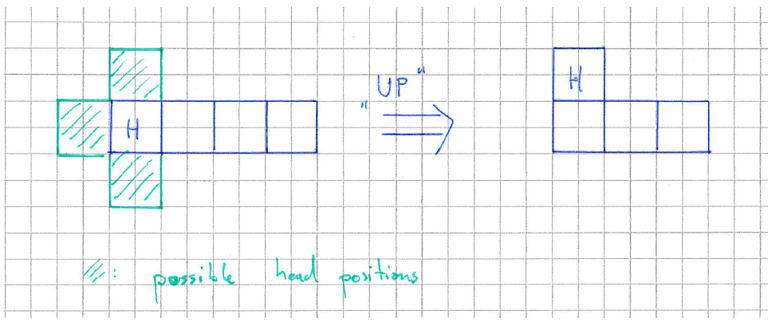
\includegraphics[scale=0.8]{snakeForward.png}
    \caption{Snake movement}
    %\label{fig:abc}
\end{figure}
\newpage The two snakes competing against each other perform their movements simultaneously. 
Furthermore, one square of the game board represents an apple. 
If a snake's head moves onto the square representing an apple, the apple disappears,
a new apple appears at a random location, and a new body element is appended to the already existing body elements. 
The new element occupies the square from which the snake's body would have just moved away. If the apple has not been reached 
after ten movements, it disappears and a new apple is created at the same time in a different place. The exact rules of when
a snake loses or wins have already been presented in Section 2.1.  . All parameters, such as the size of the game board,
starting points of the snakes, and the number of rounds, can be adjusted in the methods of the SnakesUIMain class.
 \begin{figure}[h]
    \centering
    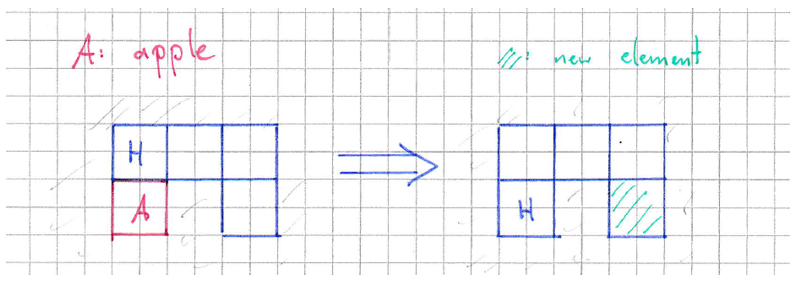
\includegraphics[scale=0.8]{SnakeApple.png}
    \caption{Snake Apple}
    %\label{fig:abc}
\end{figure}
A bot can be easily created by implementing the given interface "Bot". This interface contains a single function 
"chooseDirection" that needs to be overridden in a bot class to create a valid bot. The function has four parameters:
"Snake snake", "Snake opponent", "Coordinate mazeSize" , "Coordinate apple". "Snake" and "Coordinate" are already given 
classes. As a return value, this function has to provide a direction in which the snake's head should move in the next round.
The value of a direction is realized by the enum "Direction".\\
\\The individual squares of the game board are represented by objects of the 
"Coordinate" class, which implements the "Comparable" interface. An object of the
"Coordinate" class consists of two integer values, the x and the y component, a constructor 
and several useful methods. A very important object of this class is "mazeSize". This object 
contains the least upper bounds for the x and y values of the coordinates of the game board and 
is used, for example, to decide whether another “Coordinate”-object is inside or outside the game board.
It is initialized inside the SnakesUIMain class. Two parameters of this type are passed to 
the "chooseDirection" function - the coordinate of the apple and the already mentioned "mazeSize" object.\\
\\A snake of this game is described by an object of the "Snake" class. An object of the class "Snake"
consists of a HashSet "elements" whose elements are objects of the type "Coordinate", a deque "body"
whose elements are also objects of the type "Coordinate" and a "Coordinate" object "mazeSize", which 
should be initialized with the least upper bounds for the x and y values of the coordinates of the game
board. Various constructors and useful methods are also implemented in this class. "elements" and "body" 
of a "Snake" object contain the same values for different uses. Two parameters of this type are passed to 
the "chooseDirection" function - "Snake snake", the snake for which a direction has to be found and "Snake opponent", the opposing snake.\\
\\Based on these four parameters alone, an advantageous direction for the snake controlled by the bot 
must be found. This direction is then passed as a return value in the form of an enum "Direction" value. 
There are naturally four choices within this enumeration: Direction.UP, Direction.DOWN, Direction.LEFT,
Direction.RIGHT. These can be interpreted as directional vectors constrained to an adjacent coordinate.\\
\\A comprehensive tutorial on how to create a simple bot was also available to us on the follwing website: 
https://github.com/BeLuckyDaf/snakes-game-tutorial. We used this tutorial excessively at the first, but then 
gradually moved on and tried out our own ideas.

\section{Related Work}

In recent years, the development of artificial intelligence algorithms has seen a rapid growth,
and this growth has been particularly evident in the field of gaming. Snake, as a classic and popular game, 
has been a subject of research in the field of AI and has attracted a great deal of attention from researchers.\\
Several studies have focused on developing AI algorithms for playing Snake. For instance, reinforcement learning 
algorithms have been used to train AI agents to play Snake and improve their gameplay. Genetic algorithms have also
been applied in this context, enabling the evolution of AI agents to play Snake at a high level.\\
There has also been work on developing multi-agent systems for Snake, where multiple AI agents compete against each other.
This approach has been used to explore topics such as collaboration and competition in AI systems, as well as the development of more advanced AI algorithms.\\
There are also some other Games that implement the same Algorithm as Snake AI.\cite{RelatedWork}
\begin{itemize}
\item Flappy Bird AI
\item Breakout AI
\item Tetris AI
\item PacMan AI
\item Mario AI
\end{itemize}
For instance,Mario AI games use artificial intelligence techniques to control the actions of the character,
Mario. This can be done through techniques such as reinforcement learning, evolutionary algorithms,
or rule-based systems. The AI system receives inputs from the game environment and based on these inputs,
the AI model outputs actions for the player character, such as jumping, running and shooting.
The AI's goal is to complete the game's objectives while avoiding obstacles and enemies.
The performance of the AI is often evaluated based on metrics such as completion time, number of lives lost, and score.

\section{Proposed Approaches}
to-do
\subsection{Input/Output Format, Benchmarks (Generation, Examples)}
to-do
\subsection{Algorithms in Pseudocode}
to-do

\section{Implementation Details}
\subsection{Application Structure}
The Snake AI game consists of a interface, several classes and an enumeration, including: 
\begin{itemize}
\item Bot(Interface)
\item Direction(Enum)
\item BotLoader
\item Coordinate
\item Snake
\item SnakeGame
\item SnakeCanvas
\item SnakesRunner
\item SnakeUIMain
\item SnakesWindow
\end{itemize}

\subsection{GUI Details}
In this section, comprehensive details of all classes will be thoroughly discussed.
\subsubsection{SnakeUIMain}
This class serves as the starting point for the Snake game tournament, where several rounds of the game are conducted.
The main method of the class accepts two instances of the class Snake (snake and opponent) as arguments.\\
It is responsible for initiating rounds of the Snake game between the bots, managing I/O operations such as recording the score of the opponent and snake,
apples consumed by both snakes, and the time taken in each round. These records will be used for future statistical analysis.
\subsubsection{BotLoader}
The BoatLoader class retrieves the specified class based on its name and package from the classpath.
It enables the dynamic addition of classes to the Bot game after it has been initiated. This class inherits the abstract Java ClassLoader class.\\
A class loader is an object that is responsible for loading classes.ClassLoader is an abstract class.
When the name of a class given, a class loader should attempt to locate or generate data that constitutes a definition for the class. 
A typical strategy is to transform the name into a file name and then read a "class file" of that name from a file system.\cite{classLoader}
The only method of BotLoader class gets classBinName as argument and returns an instance of the Bot class.

\subsubsection{SnakesWindow}
The SnakesWindow class manages the graphical user interface of the game. It creates and sets up the window, runs the UI, and closes the frame when necessary. This class implements the Runnable interface.
The Runnable interface is intended for classes whose instances are meant to be executed by a thread. 
It requires the implementation of a method called 'run' that takes no arguments. The interface provides a standard protocol for objects that need to run code while active. For instance, the Thread class implements Runnable.
Being active refers to a state where a thread has been started and is yet to be stopped.\\
Moreover, Runnable allows a class to be active without requiring it to subclass Thread. A class that implements Runnable can run without subclassing Thread by instantiating a 
Thread instance and passing itself in as the target. In most cases, the Runnable interface should be used if you are only planning to override the run() method and no other Thread methods. This is important because classes should not be subclassed unless the programmer intends on modifying or enhancing the fundamental behavior of the class.\cite{runnable}
\subsubsection{SnakesRunner}
This class also implements Runnable interface and is used for running bots in a separate threads.
The Constructor of the class SnakesRunner gets running bot, snake that is controlled by the current bot,
opponent's snake, size of the board and coordinate of current position of the apple as arguments.
In addition, the chooseDirection method of the current bot is executed and saved(current direction) by this class. 
\subsubsection{SnakesGame}
The SnakesGame class implements the central gameplay flow and executes the game for two bots.
It overrides the toString() method to convert the game into a string representation and return the current game state as a string.
The randomNonOccupiedCell() method selects a random cell in the maze that is not occupied, which is used to generate a new location for the apple.
Additionally, the runOneStep() method terminates the current round if a snake takes more than one second to choose its next direction.

\subsubsection{SnakeCanvas}
The SnakeCanvas class designs the graphical user interface and enhances its appearance. It is responsible for coloring the body of the snake and opponent, making them visible on the UI.
The render() method renders the game window after filling the body of the snake, opponent and apple.
With each movement of the snake, opponent, and apple, the previously occupied positions are re-colored and marked as available for further movements.
This class inherits the Java Swing class JPanel, which is used to create various lightweight containers that can hold one or more components.
\subsubsection{Snake}
The Snake class implements the physical representation of the snakes on the game board, determining the position of snake's head, body, and length.
To achieve this, the class utilizes two efficient and logical data structures from the Java Collections framework. Each of them contains the Objects of the class "Coordinate" as elements. They are,
\begin{itemize}
\item Dequeue
\item HashSet
\end{itemize}
Those two structures contain same values, but for different purposes.
The Deque (double-ended queue) data structure allows the addition and deletion of elements from both the ends(head and tail) in $\mathcal{O}(1)$ time complexity. 
The HashSet data structure ensures basic searching, addition and deletion operations in $\mathcal{O}(1)$ time complexity .\\
This class has a important feature of cloneability which allows to copy one Object to another object without using new operator.
A class implements the Cloneable interface to indicate to the Object.clone() method that it is legal for that method to make a field-for-field copy of instances of that class.
Invoking Object's clone method on an instance that does not implement the Cloneable interface results in the exception CloneNotSupportedException being thrown.\cite{Cloneable}
\subsubsection{Coordinate}
The Coordinate class implements the position of a cell on the game board. It helps in the growth of the snake body by adding a new coordinate at the beginning of its body.
The inBounds() method ensures that the snake stays within the boundaries of the game board. This method implements the Comparable interface, making it useful in comparing two Coordinates. 
\subsubsection{Bot}
To create a working bot, all we have to do is to generate a class that implements the “Bot”-interface
The Bot interface defines a single method, chooseDirection(), which represents the decision-making process of the bot.
This method returns the direction in which the snake should move, with the options being up, down, left, or right.
\subsubsection{Apple}
Apple is an instance of the class "Coordinate".
\subsection{UML Diagram}

\begin{figure}[h]
\centering
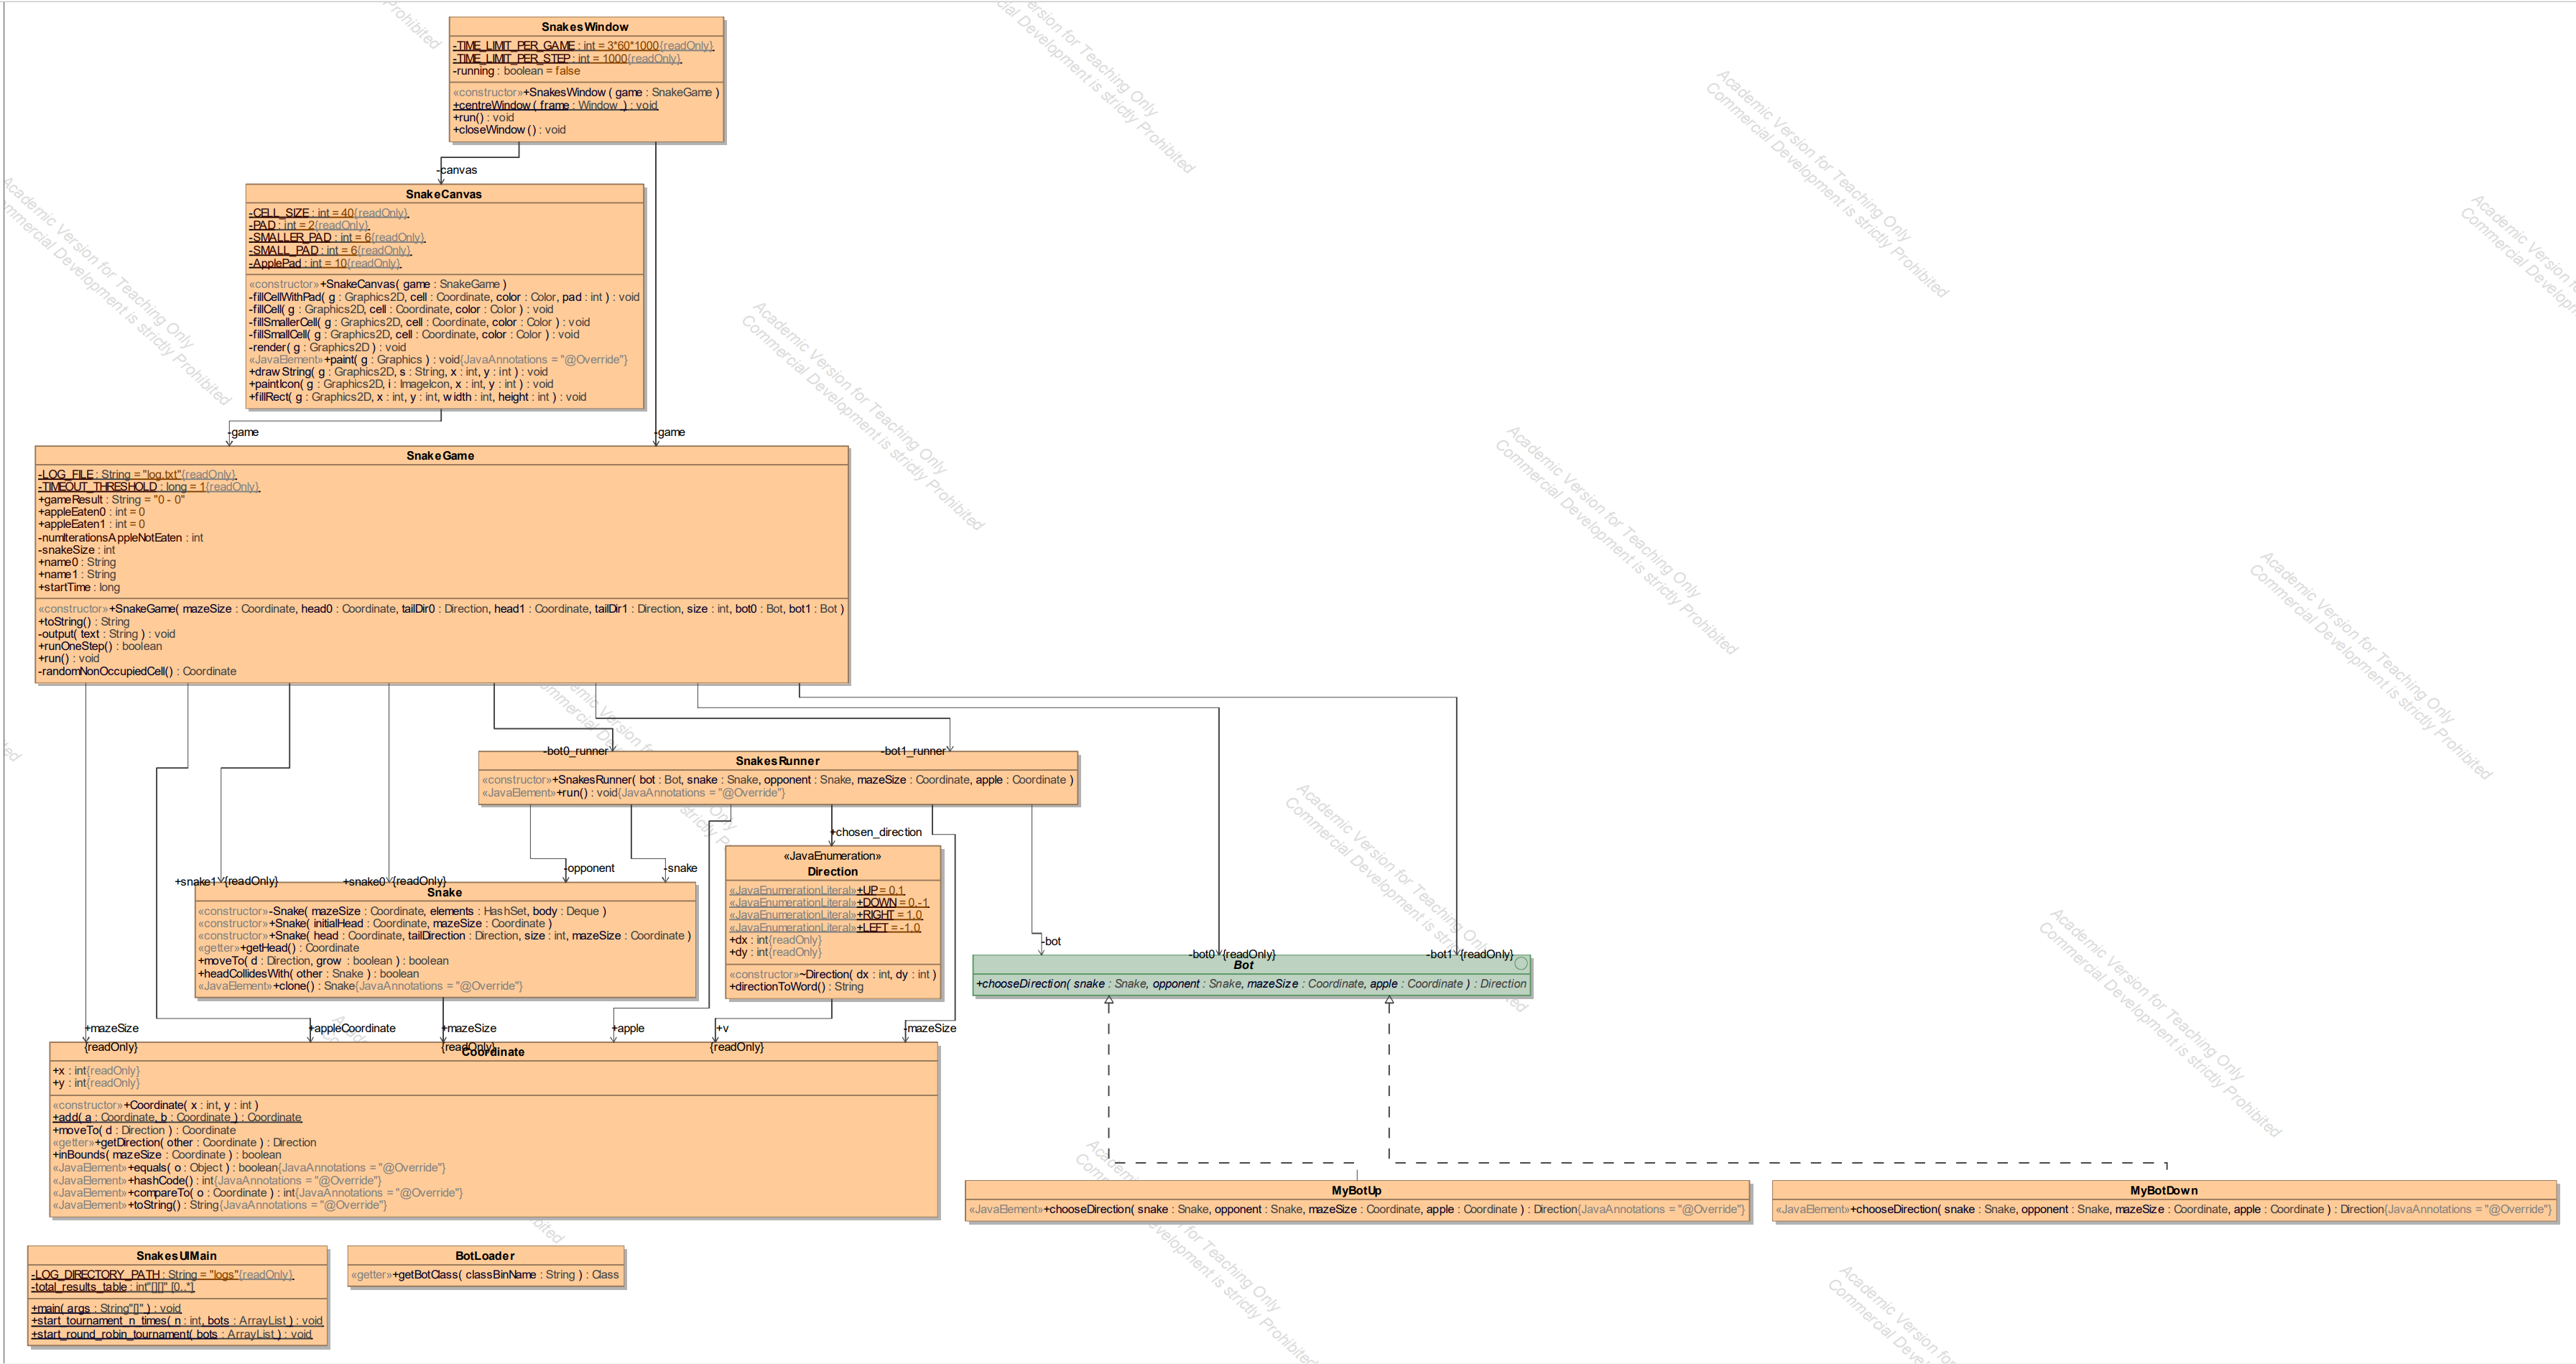
\includegraphics[scale=0.26]{ui.png}
\caption{UML diagram of the GUI}
%\label{fig:abc}
\end{figure}

\subsection{Used Libraries}
For the Developement of the Snake AI Game Java Swing Framework has been used.
Some Components from AWT framework have also been used.\\ 
Swing is a Java Foundation Classes [JFC] library and an extension of the Abstract Window Toolkit [AWT].
Swing offers much-improved functionality over AWT, new components, expanded components features, and excellent event handling with drag-and-drop support.\cite{awt}

%\subsection{Code Snippets} write code snippet with discription.
\section{Our Bots with different implementations}
\subsection{Bot1}
\title{Bot 1 (IntBot1.java):}\\
\\
After getting to know the framework of our task, one of our first objectives was implementing a
basic bot by ourselves that does the following:\\
\begin{itemize}
\item Calculate all valid moves
\item Exhibit a basic avoidance behavior regarding the opponent
\item Go for the apple
\end{itemize}
This basic bot also served as an opponent for more advanced bots later on.\\
\\
To keep things organized, we decided to create a package for each bot. The packages were created
in the „src“-folder of the given project. Each bot consists of a public class that implements the
Interface „Bot“, which as previously described, consists of only one method: „chooseDirection“.
Properly overriding this method turned this class into a bot that could be used in the game.
\\
\\
The basic idea for creating this bot was that a static array that contains all possible directions
(Direction.RIGHT, Direction.DOWN, Direction.UP, Direction.LEFT) is created outside the method
„chooseDirection“ and inside the method each element of this array is checked for its worth
concerning the stated objectives. This concept was also used in the provided example of  a bot  on the following website: \url{https://github.com/BeLuckyDaf/snakes-game-tutorial} The only thing that this bot was concerned with was not killing itself.\\
\\
Creating the static array:
\begin{minted}{java}
public class IntBot1 implements Bot {
private static final Direction[] DIRECTIONS = new Direction[]{Direction.RIGHT,
Direction.DOWN, Direction.UP, Direction.LEFT};
@Override
public Direction chooseDirection(Snake snake, Snake opponent, Coordinate
mazeSize, Coordinate apple) {
\end{minted}
The first thing we did was to create an array of possible directions of the opponent’s head and a set
that contains the resulting coordinates, so that at the end of the method „chooseDirection“ the
coordinates could be removed from the pool of possible directions of our bot’s head. To create such
an array, it was necessary to determine the coordinate of the second element of the opponent snake.
We used an iterator to achieve this in the following way:\\
\begin{minted}{java}
//Position of second Element of opponent
Coordinate afterHeadNotFinal2 = null;
if(opponent.body.size()>=2){
Iterator<Coordinate> it = opponent.body.iterator();
it.next();
afterHeadNotFinal2 = it.next();
}
final Coordinate afterHead2 = afterHeadNotFinal2;
//second element of opponent snake
\end{minted}
Note that the class „Snake“ featured a deque of elements of the „Coordinate“-class called „body“.\\
\\
After that, we used a stream method to get a sequential stream of the elements from the array
„DIRECTIONS“ to create a new array of directions called „validMovesOpponent“. The direction
whose result would equal the second element of the opponent snake was filtered out using the “equals”-method on coordinate objects. Finally, a Set of coordinates called
“possiblePositionsOpponent” was created by simply using the “moveTo” method on the head of the
opponent snake and having all elements of “validMovesOpponent” as parameters.
\begin{minted}{java}
Direction[] validMovesOpponent = Arrays.stream(DIRECTIONS)
.filter(d -> !head2.moveTo(d).equals(afterHead2))
.sorted()
.toArray(Direction[]::new);
Set<Coordinate> possiblePositionsOpponent = new HashSet<>();
for(int i=0; i< validMovesOpponent.length; i++){
possiblePositionsOpponent.add(head2.moveTo(validMovesOpponent[i]));
}
\end{minted}


Since no other restrictions were made, the set „possiblePositionsOpponent“ always contained three
elements, even if they were to be outside the maze.\\
\\
Analogous to the array „validMovesOpponent“ we created an array of directions called
„validMoves“ for our bot’s snake that excluded the possibility of backwards movement of the
snake. This array „validMoves“ was subsequently used as a parameter of the stream method to
create a new array of directions called „notLosing“, that with the use of the filter method excluded
some unfavorable outcomes.
\begin{minted}{java}
Direction[] notLosing = Arrays.stream(validMoves)
.filter(d -> head.moveTo(d).inBounds(mazeSize))
.filter(d -> !opponent.elements.contains(head.moveTo(d)))
.filter(d -> !snake.elements.contains(head.moveTo(d)))
.filter(d -> !possiblePositionsOpponent.contains(head.moveTo(d)))
.sorted()
.toArray(Direction[]::new);
\end{minted}

Using the filter method, we checked the following: Is the resulting coordinate outside the
maze? Is the resulting coordinate part of the opponent’s body? Is the resulting coordinate
part of our snake’s body? And finally, does the set „possiblePositionsOpponent“ contain the
resulting coordinate? If the answer to each of these question was „no“ the streamed element
was added to the array.\\
\\
Finally, we used the bubble sort algorithm to sort the elements of „notLosing“ based upon
the distance to the apple. „chooseDirection“ returns the first element of „notLosing“
provided that this array is not empty. If this array happens to be empty, the first element of
„validMoves“ is returned which, is never empty.
\begin{minted}{java}
//Bubble Sort; Sorting Elements of "NotLosing"
double distance1, distance2;
int a1, a2, h11, h12, h21, h22, d1, d2;
Coordinate test1, test2;
Direction temp;
if (notLosing.length > 0){
a1=apple.x;
a2=apple.y;
for(int i=0; i< notLosing.length; i++){
for(int a= i+1; a< notLosing.length; a++){
test1 = head.moveTo(notLosing[i]);
test2 = head.moveTo(notLosing[a]);
h11= test1.x;
h12 = test1.y;
d1 = (h11-a1)*(h11-a1)+(h12-a2)*(h12-a2);
distance1=Math.sqrt((double)d1);
h21= test2.x;
h22 = test2.y;
d2 = (h21-a1)*(h21-a1)+(h22-a2)*(h22-a2);
distance2=Math.sqrt((double)d2);
if(distance2<distance1){
temp=notLosing[i];
notLosing[i]=notLosing[a];
notLosing[a]=temp;
}
}
}
return notLosing[0];
}
else{
return validMoves[0];
}
}
\end{minted}
The biggest drawback of this bot was the frequent entrapment with itself or the opponent's snake. 
Even though basic evasive movements were often enough to avoid losing the game, more complex dangers like a U-shape of the opponent's
snake or the bot’s snake could not be recognized by this bot. This becomes more apparent the more elements the bodies of the snakes have.\\
\subsection{Bot2}
The concept of this Bot is based on the famous Dijkstra Algorithm which is used to determine the shortest path between two points.
In this Algorithm the following steps are performed to determine the next best possible move of the snake:
\begin{itemize}
\item finds a valid move.
\item Selects four adjacent cells(RIGHT,LEFT,UP,DOWN) from the current position(from head) of the snake.
\item Eliminates the cell that is already occupied by the snake's body(second element of snake body after head).
\item Checks if the selected move dose not lead the snake to go outside of the maze.
\item Uses the Pythagorean theorem to calculate the distance between the next position of the snake's head and the apple.
\item Determines the minimum distance among all the calculated distances.
\item Assigns the next move of the snake in the direction of the minimum distance.
\end{itemize}
To prevent collisions with the opponent snake, we have calculated all possible next moves of the opponent and stored them in a HashSet "possiblePositionsOpponent".
When determining the next move for our snake, we check if it's also the next move of the opponent.This eliminates head-to-head collisions.
\begin{minted}{java}
  //variables to find all the distances from next position of snake(head) to apple
        int disFromLeft = Integer.MAX_VALUE, disFromRight=Integer.MAX_VALUE,
		disFromUp=Integer.MAX_VALUE,disFromDown=Integer.MAX_VALUE;

        if (isValidMove(snake, mazeSize, Direction.UP, 
		(HashSet<Coordinate>) possiblePositionsOpponent,opponent)) {

            Coordinate toUp = snake.getHead().moveTo(Direction.UP);
            // find minimum distance from up to the apple using Pythagoras
            disFromUp =(int) Math.sqrt(Math.pow(toUp.x- apple.x,2)+
			Math.pow(toUp.y- apple.y,2));

        }
        if (isValidMove(snake, mazeSize, Direction.LEFT,(HashSet<Coordinate>) 
		     possiblePositionsOpponent,opponent)) {

            Coordinate toLeft = snake.getHead().moveTo(Direction.LEFT);
               // find minimum distance from left to the apple using Pythagoras
            disFromLeft =(int) Math.sqrt(Math.pow(toLeft.x- apple.x,2)+
			       Math.pow(toLeft.y- apple.y,2));

        }
        if (isValidMove(snake, mazeSize, Direction.DOWN,(HashSet<Coordinate>) 
		          possiblePositionsOpponent,opponent)) {

            Coordinate toDown = snake.getHead().moveTo(Direction.DOWN);
             // find minimum distance from down to the apple using Pythagoras
            disFromDown =(int) Math.sqrt(Math.pow(toDown.x- apple.x,2)+
			   Math.pow(toDown.y- apple.y,2));

        }
        if (isValidMove(snake, mazeSize, Direction.RIGHT,(HashSet<Coordinate>)
		      possiblePositionsOpponent,opponent)) {

            Coordinate toRight = snake.getHead().moveTo(Direction.RIGHT);
                   // find minimum distance from right to the apple using Pythagoras
            disFromRight =(int) Math.sqrt(Math.pow(toRight.x- apple.x,2)+
			      Math.pow(toRight.y- apple.y,2));
        }
       // find minimum from all the possible paths
        int minDis = Math.min(Math.min(disFromRight,disFromDown),
		       Math.min(disFromUp,disFromLeft));
            
            //give direction to the snake
        if(minDis==disFromRight){
            return Direction.RIGHT;
        } 
        else if(minDis==disFromDown){

            return Direction.DOWN;
        }
        else if(minDis==disFromLeft){

            return  Direction.LEFT;
        }
        else if(minDis==disFromUp) {
            return Direction.UP;
        }
        else{
          // to avoid worst cases.
            Random rn = new Random();
            int pos = rn.nextInt(3);
            switch (pos){

                case 0:
                    return Direction.RIGHT;
                case 1:
                    return Direction.LEFT;
                case 2:
                    return Direction.UP;
                default:
                    return Direction.DOWN;
            }
        }

\end{minted}
To determine a valid move the following additional method is used.
\begin{minted}{java}
    // evaluate a valid move
    // prevent snake to hit border of the board
    // prevent collision with the opponent
    // prevent backward movement
    boolean isValidMove(Snake snake,Coordinate mazeSize,Direction d,
	HashSet<Coordinate>opponentPos,Snake opponent){

        if(snake.getHead().moveTo(d).inBounds(mazeSize) && 
		!snake.elements.contains(snake.getHead().moveTo(d)) && 
        !opponentPos.contains(snake.getHead().moveTo(d)) && 
		!opponent.elements.contains(snake.getHead().moveTo(d))){
            //&& !opponent.elements.contains(snake.getHead().moveTo(d)
            return true;
        }
        return  false;

    }
\end{minted}
This algorithm is considered to be highly efficient in terms of its time and space complexity. 
It has a time complexity of $\mathcal{O}(1)$, meaning it runs at constant time regardless of the size of the input. 
Additionally, its space complexity is approximately $\mathcal{O}(n)$, where $n$ is the number of elements in the opponent snake's body.
The drawback of this bot was the entrapment with itself or the opponent's snake.
\subsection{Bot3}
This bot is using theorem of Pythagoras, a simplified shortest path algorithm and a kind of reversed Dijkstra which uses the longest path.\\
The bot needs to handle the following problems:
\begin{itemize}
\item avoid boundaries
\item avoid enemy snakes body
\item avoid snakes head
\item avoid himself
\item take shortest path to apple
\end{itemize}
To explain how we solved these problems let us look into the source code.
As usual we first implement the static array of directions and with that we also create a array of direction which filters with lambda functions the the valid moves.
\newpage
\begin{minted}{java}
private static final Direction[] DIRECTIONS = new Direction[] 
{ Direction.RIGHT, Direction.DOWN, Direction.UP, Direction.LEFT};
.
.
.
Coordinate head = snake.getHead();
        Coordinate oppHead = opponent.getHead();
        Coordinate afterHead = null;

        if(snake.body.size() >= 2) {
            Iterator<Coordinate> it = snake.body.iterator();
            it.next(); // first element
            afterHead = it.next(); // second element
        }

        final Coordinate afterHeadPos = afterHead;
        // avoids going backwards
        Direction[] validMoves = Arrays.stream(DIRECTIONS)
                .filter(d -> !head.moveTo(d).equals(afterHeadPos))
                .sorted()
                .toArray(Direction[]::new);
\end{minted}
So far we avoid going backwards. Now we need to handle the maze boundaries, enemies body and our snake's body. To do so we used lambda functions to filter the maze boundaries with 
".filter(d -> head.moveTo(d).inBounds(mazeSize))", filter the opponents body with ".filter(d -> !opponent.elements.contains(head.moveTo(d)))" and filter our body with ".filter(d -> !snake.elements.contains(head.moveTo(d)))".
\begin{minted}{java}
  // avoids hitting the mazebounds, opponent body, and yourself
        Direction[] notLosing = Arrays.stream(validMoves)
                .filter(d -> head.moveTo(d).inBounds(mazeSize))
                .filter(d -> !opponent.elements.contains(head.moveTo(d)))
                .filter(d -> !snake.elements.contains(head.moveTo(d)))
                .sorted()
                .toArray(Direction[]::new);
\end{minted}
However now we get to the more interesting part. The part where our snake needs to know how to decide in which direction it should go. We need to consider that our snake should take the shortest path to the apple. In theory this is really simple.\\
This is a simplified version of Dijkstra with a small graph. For further implementations we could consider not only the next 3 possible directions the snake could take, but more in depth like for the next 2 steps, 3 steps or more. This would be a great point to work on in further investigations.\\

\begin{center}
\NewAdigraph{dijkstra}
{
Left:0,0;
Head:2.5,0;
Right:5,0;
Up:2.5,2;
Apple,red:2.5,5
}
{
Head,Left:1;
Head,Right:1;
Head,Up:1; 
Left,Apple, red :12 ;
Right,Apple, red :13 ; 
Up,Apple,red: 14
}[-]
\dijkstra{}
\end{center}
%\caption{Graph of Bot3}
So first we need to know the costs of each direction to the apple. To do that we are calculating the distance by using the theorem of Pythagoras. After applying Dijkstra's algorithm to this graph, we get as result that our bot has to go to \textit{left}. The following picture will describe how we calculate the distances. We have to calculate two distances before every decision, the distance to the apple and the distance to the opponent's head.\\
\begin{figure}  
\centering
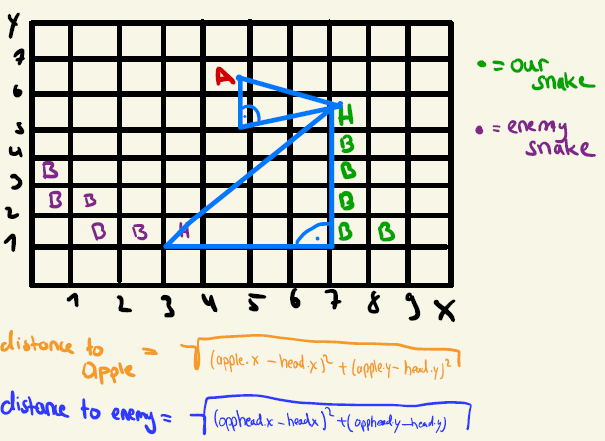
\includegraphics[scale=0.8]{calcs}
\caption{Calculations as graphical overview}
\end{figure}

\newpage
The code would look like this:
\begin{minted}{java}
//calculate the distance to other snake
double distanceToOtherSnake = 0;
   distanceToOtherSnake =  
   Math.sqrt(Math.pow((head.x - oppHead.x),2+Math.pow((head.yoppHead.y),2));
   System.out.println("Distance to other snake: " + distanceToOtherSnake);
\end{minted}
We need the distance to the other snakes head to decide whether our snake should dodge the opponents head or not. Because it only makes sense to dodge the opponent's head if it is one pixel away from our snakes head.\\
To handle the distances for each direction we used array lists. We basically calculate for each direction our snake possibly could take the  distance to the apple and to the other snakes head. You probably wonder why we should consider the distance to the enemy in this case. This is reasonable doubt but it is necessary for dodging the opponent's head. Because we take the directions which is the furthest distance to our opponent's head, to dodge his head.\\
\begin{minted}{java}
	ArrayList<Double> distancesToApple = new ArrayList<Double>();
        ArrayList<Double> distancesToOpp = new ArrayList<Double>();
        // mapping each direction of notLosing with the distance to the apple
        for (Direction dir: notLosing) {
                //calculate distances and put it in the arraylist
                int newHeadCoordinateX = snake.getHead().x + dir.dx;
                int newHeadCoordinateY = snake.getHead().y + dir.dy;
                double x = apple.x - newHeadCoordinateX;
                double y = apple.y - newHeadCoordinateY;
                double distance =Math.sqrt(Math.pow(x,2)+Math.pow(y,2));
                distancesToApple.add(distance);
                x = oppHead.x - newHeadCoordinateX;
                y = oppHead.y- newHeadCoordinateY;
                distance = Math.sqrt(Math.pow(x,2)+Math.pow(y,2));
                distancesToOpp.add((distance));
        }
\end{minted}
Now after knowing the distances our bot can look for the best directions. We are looping through our notLosing array and looking for min, max indexes of distances. So which direction is the one with the closest distance to the apple and the direction which is the furthest distance to the head of opponent.
\newpage
\begin{minted}{java}
	min = 0;
        max = 0;
        if(!distancesToApple.isEmpty())
            min = distancesToApple.get(0);
        if(!distancesToOpp.isEmpty())
            max = distancesToOpp.get(0);
         // choose the index of smallest distance
         // choose the index of furthest distance to opponents head
        for(int i = 1; i < notLosing.length; i++){
           if(distancesToApple.get(i) < min) {
               min = distancesToApple.get(i);
               indexOfMinDistance = i;
               // System.out.println(min);
           }
           if(distancesToOpp.get(i) > max){
               max = distancesToOpp.get(i);
               indexOfMaxDistanceToOpp = i;
           }
        }
\end{minted}
As last step our bot needs to decide which direction it should take based on the distance to the other snake and the possible directions of notLosing. If there is a possible direction which leads us not to die and where the distance to opponent snake's head is higher then 2 the bot takes the shortest path to the apple. If the distance to the opponents head is less or equal to 2, the bot dodges the head of the opponent. If none of these conditions met the bot just takes a valid move.
\begin{minted}{java}
	if(distancesToApple.size() > 0 && distanceToOtherSnake > 2){
            System.out.println("using shortest path");
            return notLosing[indexOfMinDistance];
        } else if ( distancesToOpp.size() > 0 && distanceToOtherSnake <= 2) {
            System.out.println("dodging opponents head");
           return  notLosing[indexOfMaxDistanceToOpp];
        } else{
            System.out.println("using valid moves");
            return validMoves[0];
        }
\end{minted}
After testing this bot and watching it for many games we noticed some problems, we also had in bots before. This bot's problem is, that it only calculates the next step. It would be more efficient to calculate more steps. With this current status the bot sometimes takes bads decisions. In some cases it takes the next closes direction to the apple and then it kills itself by hitting his own body. This is the problem of this greedy algorithm. 
\section{Experimental Results and Statistical Tests}
Like in many areas in real problems making a decision whether something is better than something else is not easy. In order to make a clearer decision, doing statistical tests and diagrams are the way to go.\\
Doing 5 games and deciding if a bot is better than the other one would be a misguided decision. This is comparable to the Law of Large Numbers. If you have a coin, which is equally like that head or tail shows. The probability that head or tail shows is for both 50\%(0.5). If you know take the coin and toss it 10 times. If the result is 8 times head and 2 time tail you can't state correctly from your experiment that the probability is now for head 80\%(0.8) and for tail 20\%(0.2). Doing the same experiment 1000 times will show that the average chance to hit head or tail gets really close to 50\%.\\
This is similar to our scenario. If we would let the bots play for 5 rounds and one snake is winning 4 times and the other 1 time you can't tell directly that the one who had more wins in this 5 rounds is the better snake. There are chances that the apple spawns in bad positions. So to tell whether a bot is better than a other bot we want to let them play 1000 times and then compare the wins. We also want to show statistical the average score, apple's eaten and time played. In the following you will see the results of our tests.\newpage
\subsection{Simulations (Play with the Parameters!)}
First of all we need to dive into the code. The standard amount of rounds played is set to 5. To change that we navigated to the SnakesUIMain where you can setup the amount of rounds.
\begin{minted}{Java}
start_tournament_n_times(5, bots);
\end{minted}
Changing the first parameter to 1000 will let them play 1000 times against each other. The framework uses .txt files to track the games. The folder structure, after setting the parameter to 10 and letting the bots play, looks like:

\begin{center}

\includegraphics[scale=0.8]{logs_structure}
\end{center}
%\caption{Logs_structure.png}

The "iteration\_i.txt" file logs the data for each round. The "total.txt" file logs the summary of all rounds. The content of those files are structured like this:\\
\\
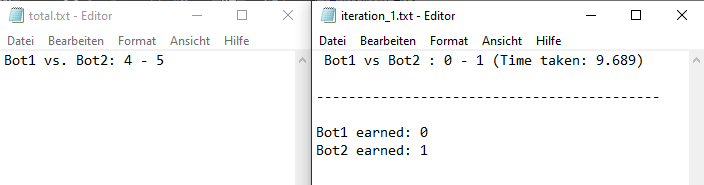
\includegraphics[scale=0.8]{logs_content}
\\For our statistical tests these information are not sufficient and not structured well. So we need a new file structure. First of all we need to think about what we really want to show and which variables we want to use. We need a variables like round , type of bot, results, apples eaten, time played. Round describes the round number. Type of bot describes which bot is meant (e.g. 1 for the first bot 2 for the second bot). Apples eaten for each bot so how many apple they ate in that round. The other ones are trivial so we don't need any further explanations. An example entry would look like: 3,1,2,0,1,7,13,30.45
\\ This would show the third round where the second bot has won. The first bot ate 7 and the second bot ate 13 apples. The round ended after 30.45 seconds.
\subsection{Use Benchmarks}
to-do
\subsection{Tables: input data details, results of different algorithms}
to-do
\subsection{Charts}
to-do
\subsection{Evaluations}
to-do

\section{Conclusions and Future Work}
We started our project with a small amount of knowledge and now we know more about algorithms in field of Artificial Intelligence. Our beginning was hard because not everything was clear. But we managed to meet weekly and talk about problems and new findings. Every meeting made our visions of this project clearer. Our goal was to make multiple bots and to compete them against each other. Back then we started with implementing basic algorithms. Afterwards we observed benefits and drawbacks of the algorithms we used. Then we worked again on them to improve them. To decide which one of the final algorithms were the best one, we made statistical tests. We collected data and then made a data analysis. Out of that data analysis we could decide, that the best bot was the recursive-bot \ref{RecursiveBot}. We had a lot of fun while working on this project.
\subsection{How the team work went}
Talking about the team work, communication was our keyword to success. If any team member had problems we assembled and helped out each other. We held meetings in the university and also meetings via Discord. Discord is a online service where people can join servers and talk with each other, share files and chat with each other. We made a server for this project. Where we uploaded sometimes files, but for the most time we used it for holding our meetings. Our version control was done with GitHub.\\
We were able to find a time slot where we could meet. This made it easier for us to work on the documentation and algorithms. The benefit was definitely the group size. The more persons in the group , the more difficult it gets to find a schedule where everyone has time for.
\subsection{What we have learned}
We have learned a lot about pathing algorithms. It also made us clear how important it is to have algorithms, like Dijkstra, which returns us the shortest path. While working out, where we could use it in real life, we realized that we are facing these algorithms daily.  In navigation and social media apps e.g.
This project taught us not only how to implement efficiently working algorithms, but also to work in a team. We learned that we have to talk about our problems. Not only problems in development, also psychological problems. It was a tough time for all of us, because we had a strict schedule and many modules to study for. We helped each other in both of the problems, so we were motivated to work on this project even more. We found a good sense for distributing the work, which also made the work in total easier.\\

\subsection{Ideas for the future development of your application, new algorithms}
to-do
\bibliography{bibliography}
\bibliographystyle{plain}
\end{document}